\documentclass[11pt]{article} % 11-pt font size
\usepackage{titling}
\usepackage[left=1in, right=1in, top=1in, bottom=1in]{geometry}  % Set 1-inch margins
\usepackage{multicol} % Include the multicol package
\usepackage{graphicx} % Required for inserting images
\usepackage{enumitem} % Cleaner package for numbering 
% \usepackage[style=apa, backend=biber]{biblatex} % Package for references APA
\usepackage{hyperref} % For clickable links
\usepackage[english]{babel}
\usepackage[utf8x]{inputenc}
\usepackage{amsmath}
\usepackage{graphicx}
\graphicspath{{Images/}}
\usepackage{float}
\usepackage[colorinlistoftodos]{todonotes}
\usepackage{booktabs}
\usepackage{subcaption}
\usepackage{listings}
\usepackage{hyperref}
\usepackage{tabularray}
\usepackage{amssymb}
\usepackage{hyperref}
\begin{document}
    \begin{titlepage}
    
    \newcommand{\HRule}{\rule{\linewidth}{0.5mm}} % Defines a new command for the horizontal lines, change thickness here
    
    \center % Center everything on the page
    %----------------------------------------------------------------------------------------
    %	HEADING SECTIONS
    %----------------------------------------------------------------------------------------
    
    \textsc{\LARGE Georgia Institute of Technology}\\[1.5cm] % Name of your university/college
    \includegraphics[scale=.6]{images/GeorgiaTech_RGB.png}\\[1cm] % Include a department/university logo - this will require the graphicx package
    
    %----------------------------------------------------------------------------------------
    %	TITLE SECTION
    %----------------------------------------------------------------------------------------
    
    \HRule \\[0.4cm]
    { \huge \bfseries Ryan Air - Passenger Reviews Analysis}\\[0.4cm] % Title of your document
    \HRule \\[1.5cm]
    
    \textsc{\Large ISYE 6740 -  Computational Data Analysis}\\[0.5cm]
    \textsc{\large \textbf{ISYE 6740 Project Group 114}}\\[0.6cm]
    {\large \today}\\[2cm]
    \begin{center}
    \begin{minipage}{0.33\textwidth}
        \centering
        {\Large Ashish Puri} \\
        apuri61@gatech.edu \\
        GTID:XXXXXX582
    \end{minipage}%
    \begin{minipage}{0.33\textwidth}
        \centering
        {\Large Jagannath Banerjee} \\
        jbanerjee7@gatech.edu \\
        GTID:XXXXXX232
    \end{minipage}
    \begin{minipage}{0.33\textwidth}
        \centering
        {\Large Piyush Shivrain} \\
        pshivrain3@gatech.edu \\
        GTID:XXXXXX723
    \end{minipage}
    \end{center}
\end{titlepage}

\section{Problem Statement}
In contemporary business landscapes characterized by a paramount emphasis on customer feedback, the aviation sector stands as no exception. Amidst the burgeoning influx of online reviews, the conventional manual analysis of textual data becomes both impracticable and resource-intensive. Consequently, our project endeavors to confront this challenge through a programmatic framework, harnessing the capabilities of Natural Language Processing (NLP) techniques. By employing methodologies encompassing data exploration, sentiment classification, and topic modeling, this project aims to dissect passenger reviews comprehensively. Moreover, the study aspires to undertake root cause analysis to discern the foremost challenges encountered by passengers, along with delineating the specific routes most afflicted by these challenges.  \\
\\
In this project, we aim to conduct a comprehensive analysis of passenger experience reviews for
Ryanair, spanning from 2012 to 2024. Ryanair is one of Europe’s leading low-cost airlines that garners a vast amount of feedback from its passengers, covering various facets of their travel experience. Analyzing passenger reviews can offer Ryanair valuable insights into various aspects of their services, operations, and customer experiences.\\\\
The project aims to achieve several objectives:
\begin{itemize}
    \item \textbf{Overall Sentiment Analysis:} Evaluate the overall sentiment of passengers towards airline services, exploring their satisfaction levels across the entirety of their travel experience.
    \item \textbf{Service Quality Assessment:} Identify specific services or amenities that evoke the highest levels of satisfaction or dissatisfaction among passengers. Additionally, pinpoint recurring issues or patterns across reviews to understand service quality comprehensively.
    \item \textbf{Operational Aspect Scrutiny:} Investigate frequent complaints or commendations regarding customer service, flight punctuality, baggage handling, and check-in procedures. Identify routes or flights consistently receiving negative feedback concerning operational aspects.
    \item \textbf{Customer Service Evaluation:} Examine passengers' perceptions of the responsiveness and helpfulness of airline staff, both on the ground and during flights. Identify instances of exceptional or poor customer service mentioned in reviews.
    \item \textbf{Sentiment Classifier Development:} Develop a sentiment classifier using machine learning techniques specifically tailored to Ryanair's context. This classifier will aid in automatically categorizing and analyzing passenger sentiments from reviews.
\end{itemize}
\textbf{Innovation:}In our paper, we showcase our ability to pinpoint and address negative sentiments by tracing them back to specific airline routes leveraging graph network visualization and illustrate the routes with root cause.
\section{Data Source}
The dataset from Kaggle \href{https://www.kaggle.com/datasets/cristaliss/ryanair-reviews-ratings?resource=download}{Ryan air passenger review}provides a comprehensive collection of passenger reviews and ratings focusing on their experiences with Ryanair, a prominent low-cost airline operating in Europe. Dataset contains 2249 rows and 21 columns.Spanning from 2012 to 2024, this dataset encompasses a diverse range of insights, including passenger-reported ratings on various aspects such as seat comfort, cabin crew service, food and beverages, ground service, and overall value for money. Additionally, it offers detailed information about the types of travelers, such as leisure, business, or family, as well as details on aircraft types, seat types, routes flown, dates of travel, passenger nationalities, and trip verification status. Each column provides valuable information for analysis:
% Data Table Here
\begin{table}[H]
\begin{tabular}{@{}ll@{}}
\toprule
{\color[HTML]{343434} \textbf{Column}}          & \textbf{Details}                                                         \\ \midrule
{\color[HTML]{343434} Date Published}           & The date when the review was   published                                 \\
{\color[HTML]{343434} Overall Rating}           & Numeric ratings provided by   passengers for their overall experience    \\
{\color[HTML]{343434} Passenger   Country}      & The country of origin of the   passenger                                 \\
{\color[HTML]{343434} Trip   verified}          & Indicates whether the trip has   been verified                           \\
{\color[HTML]{343434} Comment   title}          & The title or header of the review                                        \\
{\color[HTML]{343434} Comment}                  & The main body of the review,   containing detailed comments and feedback \\
{\color[HTML]{343434} Aircraft}                 & The type of aircraft used for the   flight                               \\
{\color[HTML]{343434} Type   Of Traveller}      & The type of traveler, such as   leisure, business, or family             \\
{\color[HTML]{343434} Seat   Type}              & The type of seat booked for the   flight                                 \\
{\color[HTML]{343434} Destination}              & The destination of the flight                                            \\
{\color[HTML]{343434} Date   Flown}             & The date when the flight took   place                                    \\
{\color[HTML]{343434} Seat   Comfort}           & Ratings for seat comfort provided   by passengers                        \\
{\color[HTML]{343434} Cabin   Staff Service}    & Ratings for cabin staff service   provided by passengers                 \\
{\color[HTML]{343434} Food   \& Beverages}      & Ratings for food and beverages   provided by passengers                  \\
{\color[HTML]{343434} Ground   Service}         & Ratings for ground services   provided by passengers                     \\
{\color[HTML]{343434} Value   For Money}        & Ratings for overall value for   money provided by passengers             \\
{\color[HTML]{343434} Recommended}              & Indicates whether the passenger   would recommend the airline            \\
{\color[HTML]{343434} Inflight   Entertainment} & Ratings for inflight entertainment   provided by passengers              \\
{\color[HTML]{343434} Wifi   \& Connectivity}   & Ratings for wifi and connectivity   provided by passengers               \\ \bottomrule
\end{tabular}
\end{table}
\section{Methodology}
\subsection{Data Preparation}
Customer reviews often contain noisy text, including spelling errors, grammatical mistakes, slang, abbreviations, and emoticons. For our analysis, data preparation was a key step. For Pre-processing steps, we explored the structure of the dataset - checked columns, data types, and any missing values and dropped rows with no reviews and ratings.Subsequently, we removed irrelevant features that won't contribute to the analysis like Unnamed: 0, Passenger Country and Type of Traveller.Next, we converted the data to lowercase, tokenized, removed punctuation, emoticons, urllinks and stopwords, and lemmatized the data.

\subsection{Exploratory Data Analysis (EDA)}
For exploratory data analysis, we visualized the sentiment distribution, review lengths, temporal trends, and linguistic patterns. Initially, we delved into the distribution of review ratings on the prevalence of positive, negative, and neutral sentiments. Next, we analyzed the distribution of review lengths across sentiment categories, aiming to discern any correlations between sentiment and review length. Moreover, we conducted a temporal analysis to unveil sentiment trends over time, potentially uncovering seasonal patterns or shifts in sentiment dynamics. Additionally, we employed techniques such as word cloud generation to elucidate the most frequent words and phrases used in reviews. Furthermore, we identified routes associated with the most negative feedback, pinpointing areas for potential improvement using graph visualization. Lastly, we performed bi-gram analysis for negative sentiments to identify the most frequent word combination occurring together.

\subsection{Sentiment Analysis}
We employed \href{https://spacy.io/universe/project/spacy-textblob}{TextBlob sentiment analysis pipeline component from spaCy} to label the reviews into positive, negative and neutral—expressed within each reviews and calculate their sentiment polarity score. Spacy provides the following components to identify the sentiments.
\begin{verbatim}
doc..blob.polarity
doc..blob.subjectivity
doc._.blob.sentiment_assessments.assessments 
\end{verbatim}

\texttt{doc.\_.blob.polarity}:Represents the polarity of the text, indicating whether the sentiment expressed in the document is positive, negative, or neutral. Polarity is a numerical value ranging from -1 (negative) to 1 (positive), with 0 indicating neutral sentiment. For example, a polarity of -0.125 suggests slightly negative sentiment.

\texttt{doc.\_.blob.subjectivity}: Subjectivity refers to the degree to which the text expresses personal opinions, feelings, or beliefs rather than factual information. The subjectivity score ranges from 0 to 1, with higher values indicating more subjective text. A subjectivity score of 0.9 suggests that the text is highly subjective, likely containing personal opinions or emotions.

\texttt{doc.\_.blob.sentiment\_assessments.assessments}: provides detailed assessment of sentiment within the text, including individual assessments for each sentiment-bearing phrase or word. Each assessment consists of a tuple containing the sentiment-bearing words or phrases, their polarity score (ranging from -1 to 1), their subjectivity score (ranging from 0 to 1), and additional metadata (such as the context of the assessment). For example, the assessments `(['really', 'horrible'], -1.0, 1.0, None)` and `(['worst', '!'], -1.0, 1.0, None)` indicate that the words "really horrible" and "worst" (followed by an exclamation mark) are associated with strongly negative sentiment, with polarity scores of -1.0 and subjectivity scores of 1.0.

These components provide valuable insights into the sentiment expressed in text documents, allowing for automated analysis and interpretation of textual data in various NLP applications.
\subsection{Topic Modeling}
In our analysis of customer reviews, we applied topic modeling technique called Latent Dirichlet Allocation (LDA) to understand underlying themes and topics within the textual data. \\


The Latent Dirichlet Allocation (LDA) model represents each document \( w \) as a mixture over latent topics, characterized by a distribution \( \theta \). This generative process is governed by the following steps: first, a Poisson distribution is chosen for the document length, then a document-topic distribution \( \theta \) is sampled from a Dirichlet distribution \( \text{Dir}(\alpha) \), and finally, for each word in the document, a topic \( z \) is chosen from a multinomial distribution defined by \( \theta \), and a word is chosen from a multinomial distribution conditioned on the selected topic. Mathematically, this process is represented as:
\[
\theta_d \sim \text{Dir}(\alpha)
\]
\[
z_{dn} \sim \text{Mult}(\theta_d)
\]
\[
w_{dn} \sim \text{Mult}(\phi_{z_{dn}})
\]

The joint distribution of a topic mixture \( \theta \), a set of topics \( z \), and a set of words \( w \) is given by:
\[
p(\theta, z, w | \alpha, \beta) = p(\theta | \alpha) \prod_{n=1}^{N} p(z_n | \theta) p(w_n | z_n, \beta)
\]

The probability of a corpus is obtained by integrating over \( \theta \) and summing over \( z \):
\[
p(w | \alpha, \beta) = \int p(\theta | \alpha) \left( \prod_{n=1}^{N} \sum_{z_n} p(z_n | \theta) p(w_n | z_n, \beta) \right) d\theta
\]

The LDA model is represented as a graphical model with three levels: corpus-level parameters \( \alpha \) and \( \beta \), document-level variables \( \theta \), and word-level variables \( z \) and \( w \). The key inferential problem in LDA involves computing the posterior distribution of the hidden variables given a document, which is generally intractable to compute exactly. Approximate inference algorithms, such as variational inference or Markov chain Monte Carlo, are often employed to address this challenge.\\




By identifying recurring sets of words that co-occur within the reviews, we discerned the most pertinent topics discussed by customers, providing valuable insights into prevalent themes. Our focus extended to topics associated with negative sentiment, targeting specific issues commonly cited in negative reviews, such as "poor customer service," "delayed flights," and "uncomfortable seats.". Additionally, we assessed the prevalence of each negative sentiment topic by analyzing its frequency of occurrence across the dataset, thereby identifying significant pain points likely to impact customer satisfaction and informing strategic decision-making processes accordingly. \\





\underline{Hyperparameter Tuning:}
LDA has two hyperparameters: $\alpha$ and $\beta$. $\alpha$ controls the document-topic sparsity, while $\beta$ controls the topic-word sparsity. Mathematically, this can be represented as:
\[
\begin{aligned}
\theta_d & \sim \text{Dir}(\alpha) \\
\phi_k & \sim \text{Dir}(\beta) \\
z_{dn} & \sim \text{Mult}(\theta_d) \\
w_{dn} & \sim \text{Mult}(\phi_{z_{dn}})
\end{aligned}
\]
$\alpha$ and $\beta$ are tuned within specified ranges. Coherence score (\textit{coherence score}) is calculated for each configuration.

\underline{Model Selection:}
The configuration with the highest coherence score is selected as the final model. Mathematically, this can be represented as:
\[
\text{coherence score} = f(\text{alpha}, \text{beta}, \text{topic})
\]
where \textit{topic} refers to the number of topics.









\underline{Final Configuration:}
For our model, the chosen configuration is:
$\alpha = 0.5$, $\beta = \text{auto}$, which provided highest coherence score and gave us the number of  $\text{topics} = 10$






\subsection{Sentiment Classifier}
For sentiment classification, we used 3 variants of Naive Bayes classifiers - Complement NB, Multinomial NB, and Bernoulli NB.Naive Bayes classifiers are well-suited for handling text data, which is inherently sparse and high-dimensional. They work effectively with bag-of-words or bag-of-ngrams representations, making them suitable for sentiment analysis tasks where feature extraction from text is crucial.Naive Bayes classifiers are computationally efficient and can scale well to large datasets and are robust to irrelevant features or noisy data.\\
\textbf{Complement Naive Bayes}:CNB is an adaptation of the standard multinomial naive Bayes (MNB) algorithm that is particularly suited for imbalanced data sets. CNB uses statistics from the complement of each class to compute the model’s weights.The formula for weight calculation in Complement Naive Bayes (CNB) is derived from the multinomial distribution and accounts for class imbalance. In CNB, instead of directly computing the probability of each feature given the class as in traditional Naive Bayes, the complement class is considered. This is particularly useful for imbalanced datasets, where some classes may have significantly more instances than others. The weight \( \theta_{ic} \) for feature \( i \) in class \( c \) is calculated as follows:

\[ \theta_{ic} = \frac{{\alpha + \sum_{d \neq c} {n_{id}}}}{{\alpha \cdot N + \sum_{d \neq c} {\sum_i {n_{id}}}}}\]

Where \( \alpha \) is a smoothing parameter (usually set to 1), \( n_{id} \) is the frequency of feature \( i \) in documents of class \( d \) and
\( N \) is the total number of training instances.
\\
\\
\textbf{Multinomial NB}: MultinomialNB, a variant of the naive Bayes algorithm, is tailored for analyzing multinomially distributed data, making it ideal for text classification tasks. In text classification, documents are often represented as word vectors, where each element of the vector corresponds to the count of a specific word in the document.

The algorithm's key parameterization involves vectors $\boldsymbol{\theta}_y = (\theta_{y1}, \ldots, \theta_{yn})$ for each class $y$, where $n$ represents the number of features, typically reflecting the vocabulary size. Here, $\theta_{yi}$ denotes the likelihood of feature $i$ appearing in a document belonging to class $y$.

These parameters are estimated using a smoothed version of maximum likelihood, expressed by the formula:

\[
\hat{\theta}_{yi} = \frac{N_{yi} + \alpha}{N_{y} + \alpha n}
\]

In this formula:

$N_{yi}$ represents the count of feature $i$ occurring in documents of class $y$ in the training set.

$N_{y}$ is the total count of all features for class $y$.

$\alpha$ is a smoothing parameter that handles features absent in the training samples and prevents zero probabilities in calculations.
\\
\\
\textbf{Bernoulli NB}: BernoulliNB, a variant of the naive Bayes algorithm, is specialized for data following multivariate Bernoulli distributions, where features are binary-valued (true/false). It operates on binary feature vectors and may transform input data accordingly.

Its decision rule, unlike that of multinomial NB, incorporates an explicit penalty for the absence of a feature indicating a class $y_i$. This is expressed by the formula:

\[
P(x_i \,|\, y) = P(x_i = 1 \,|\, y) \cdot x_i + (1 - P(x_i = 1 \,|\, y)) \cdot (1 - x_i)
\]

In text classification, it's common to employ word occurrence vectors instead of word count vectors with BernoulliNB. This model may offer superior performance on datasets with shorter documents.
\subsection{Exploratory Data Analysis (EDA)}
We explored passenger rating (1-Low, 5-High) across various aspects of services provided by the airline as shown below and found rating 1 dominating the most.Usually, passengers with bad experiences are more inclined to write a review.
\begin{figure}[H]
    \centering
    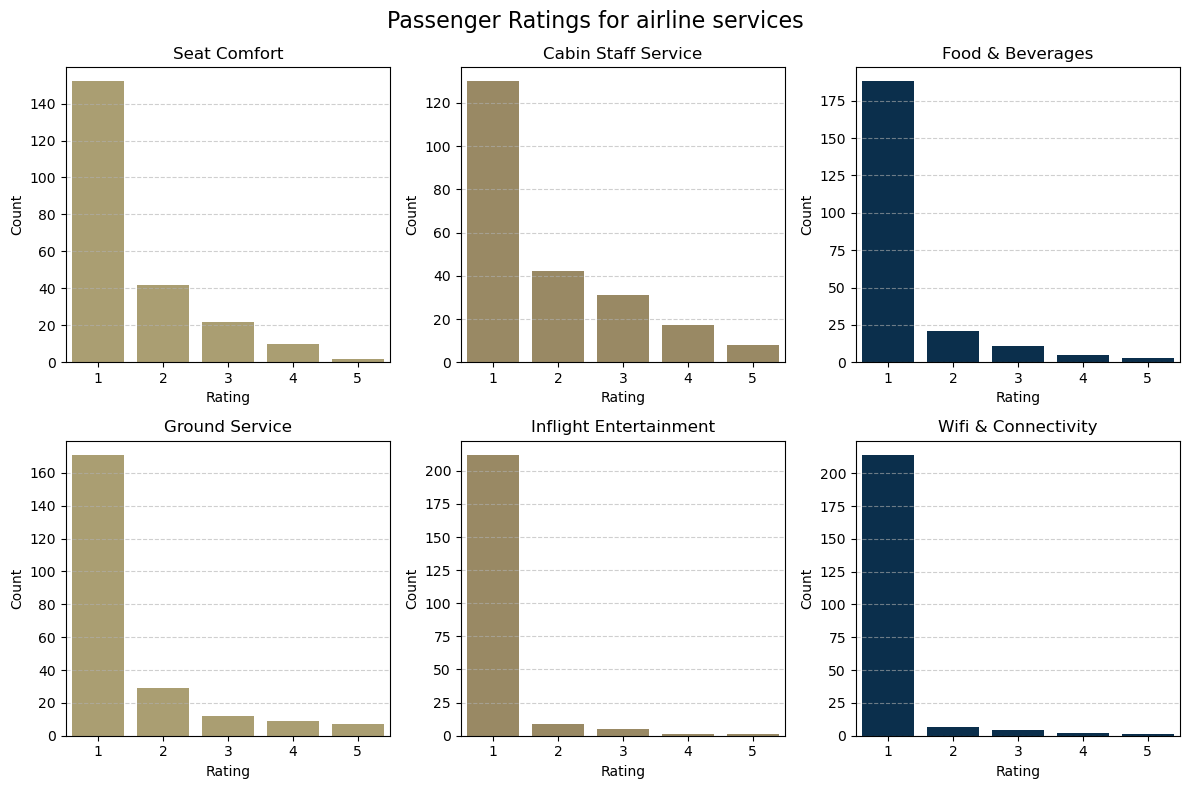
\includegraphics[width=0.7\textwidth]{images/images/review_ratings.png}
    \caption{Customer Ratings across various services}
    \label{fig:Customer Ratings across various services}
\end{figure}
\subsection{Sentiment Analysis}
Using Spacy sentiment analyzer, we estimated the sentiment for each review into three categories (positive, negative, and neutral). Here we observe that the overall number of positive reviews is almost double the number of negative reviews. This is in stark contrast to what we observed when we looked at the ratings given to various flight experiences such as seating, service, etc. 
Further, we analyzed the length of review for positive and negative sentiments and found the majority of positive reviews hovered around 150 words while negative reviews hovered around the 100-word mark, suggesting positive review having more words.
\begin{figure}[H]
  \centering
  \begin{subfigure}[b]{0.4\textwidth}
    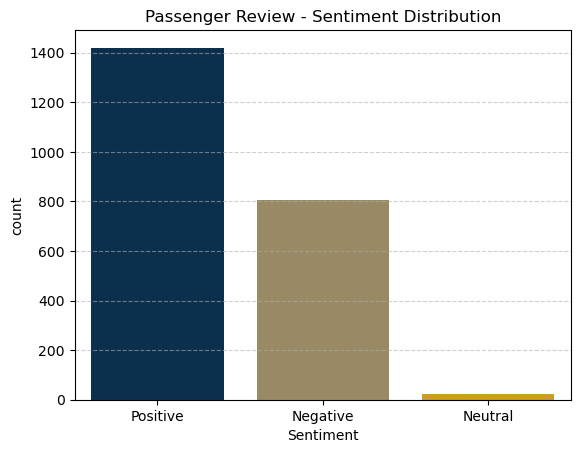
\includegraphics[width=\textwidth]{images/sentiment_distribution.png}
    \caption{Sentiment Analysis of all reviews}
    \label{fig:sub1}
  \end{subfigure}
  \hfill
  \begin{subfigure}[b]{0.5\textwidth}
    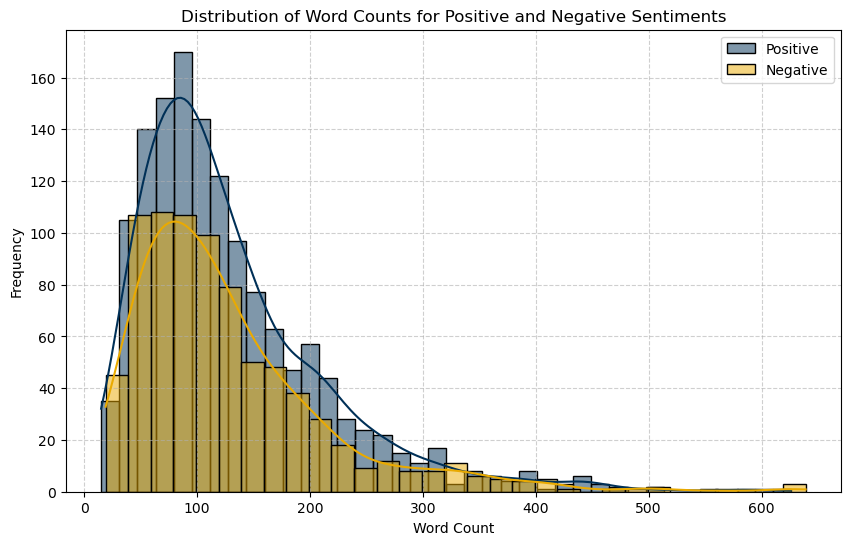
\includegraphics[width=\textwidth]{images/distribution_review_length.png}
    \caption{Word count distribution of Positive \& Negative sentiments}
    \label{fig:sub2}
  \end{subfigure}
  \caption{Sentiment Analysis \& Word Count distribution for each sentiments}
\end{figure}
Next, we visualized the temporal trends ie, patterns and changes in sentiment over time.Long-term temporal trends provide insights into overall shifts in sentiment over extended periods, such as months or years.Short-term temporal trends capture transient changes in sentiment may be influenced by specific events, news stories, marketing campaigns, or social media trends. We observe highest negative sentiments during year 2018 and 2019. Then the reviews significantly decreased may be due to Covid till 2022.2018 and 2019 will be interesting year to review.We also observe that July, September and October has highest negative comments. It could be due to a high travel season between summer and fall.
\begin{figure}[H]
  \centering
  \begin{subfigure}[b]{0.45\textwidth}
    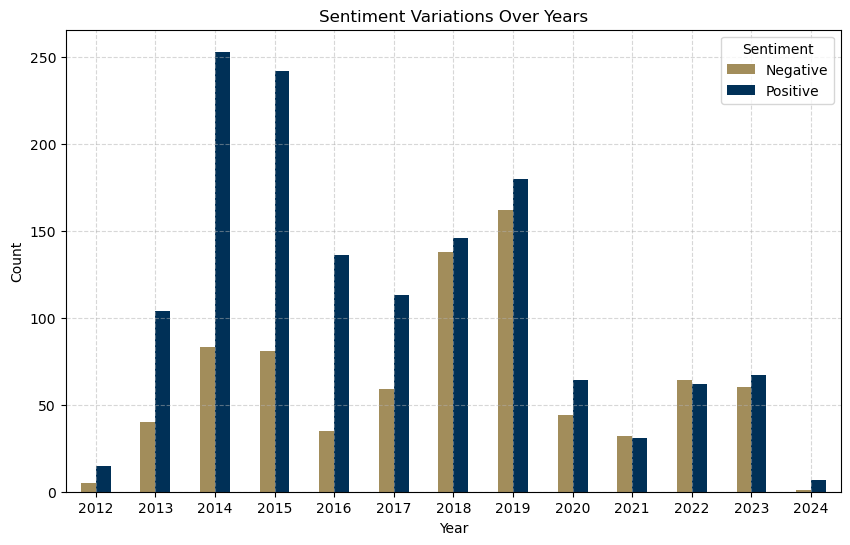
\includegraphics[width=\textwidth]{images/sentiment_variation_over_year.png}
    \caption{Temporal Trend over Year}
    \label{fig:Temporal Trend over Year}
  \end{subfigure}
  \hfill
  \begin{subfigure}[b]{0.45\textwidth}
    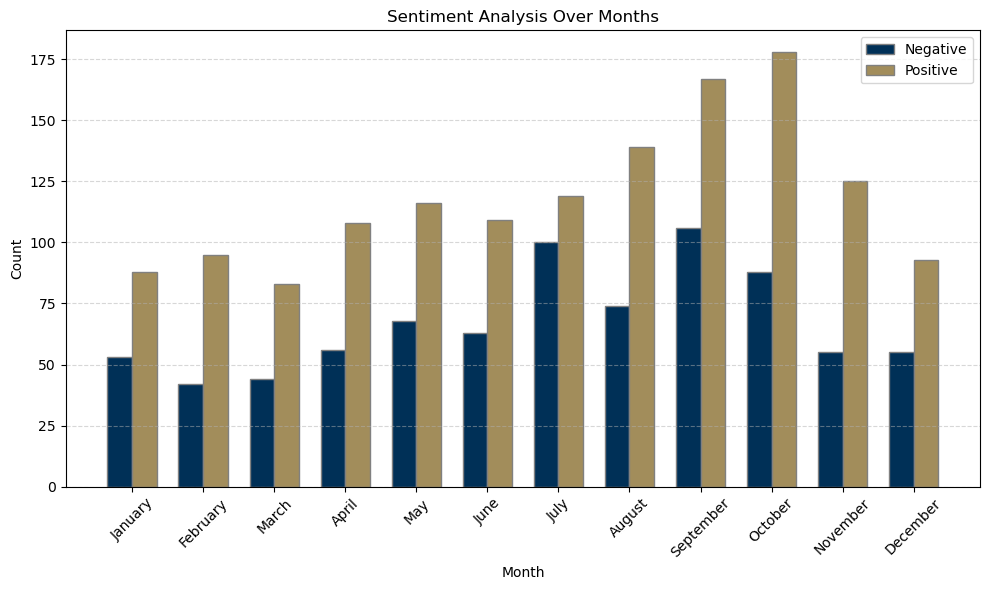
\includegraphics[width=\textwidth]{images/sentiment_variation_over_month.png}
    \caption{Temporal Trend by Month}
    \label{fig:Temporal Trend by Month}
  \end{subfigure}
  \caption{Temporal Trend over Time}
  \label{fig:twosidebyside}
\end{figure}
To comprehend the prevailing sentiments within negative reviews, we analyzed the linguistic characteristics embedded within the text using word cloud. Through word cloud, were able to understand that the high level concerns and grievances are expressed around customer service, uncomfortable seat, airline staff, terrible service and strong use of words like awful, worst experience, disappointed, never fly, worse etc. Also customers are taking about 2 airports - Dublin and Stansted. We will explore deep into these issues and routes to understand more.
\begin{figure}[H]
    \centering
    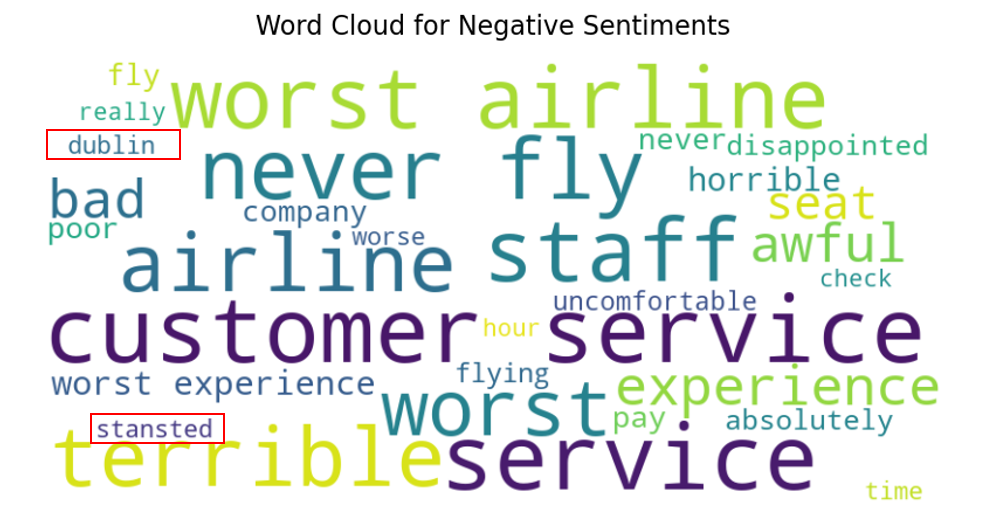
\includegraphics[width=0.7\textwidth]{images/word_cloud_freq_words_v1.png}
    \caption{Word Cloud of Negative Comments}
    \label{fig:Word Cloud of Negative Comments}
\end{figure}

\subsection{Topic Modeling}
We took the negative sentiments and performed topic modelling using  Latent Dirichlet Allocation (LDA) to understand the underlying themes and topics discussed by customers. Here we identified the clusters of words that frequently co-occur within the reviews. In the below representation, the bubbles in PC1 and PC2 (Principal Component 1 and Principal Component 2) represent topics in the topic space.We have selected 10 topics each representing a cluster of words constituting a topic.Proximity of bubbles represents the closeness of each topic from another. In this case, we have selected \textbf{topic 3} which is distinctly separate from others and observed that it talks about \textbf{customer service} and airport \textbf{Dublin}.Using the below topic modelling, we will explore 2 areas - Topic\# 3 having Poor Customer Service from Dublin and Topic\# 8 having uncomfortable seats from Stansted.
\begin{figure}[H]
    \centering
    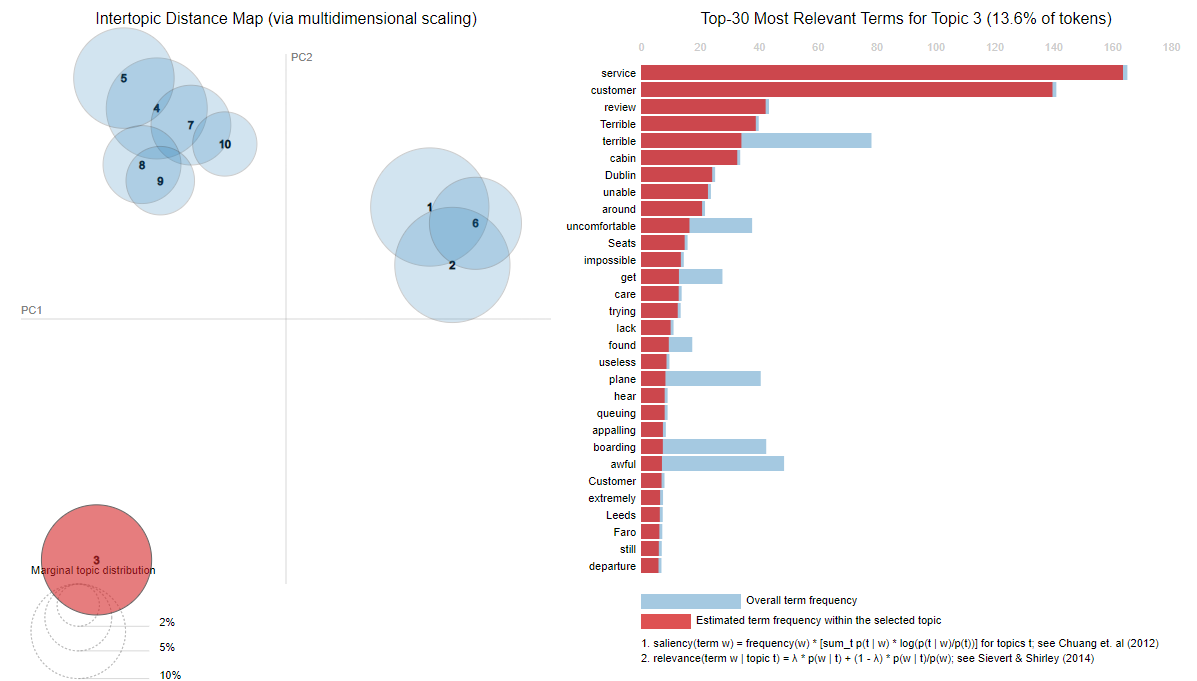
\includegraphics[width=0.75\textwidth]{images/lda_topic_model_3.png}
    \caption{Bi-gram Analysis}
    \label{fig:Bi-gram Analysis}
\end{figure}
Below are the words with highest frequencies within each topics:
\begin{table}[H]
\centering
\begin{tabular}{@{}cl@{}}
\toprule
\multicolumn{1}{l}{\textbf{Topic}} & \textbf{Relevant Terms}                                      \\ \midrule
1                                  & Never Fly, Boarding,   Awful                                \\
2                                  & Terrible Experience, Bad Food, Horrible, Shocking            \\
3                                  & \textbf{Customer Service, Dublin, Terrible, Worst, Shocking} \\
4                                  & \textbf{Poor Staff, time, ticket,   luggage}                 \\
5                                  & Filthy, Unpleasant, Seat, Luggage, Aweful                    \\
6                                  & Worst Airline, Worst ever                                    \\
7                                  & \textbf{Online Ticket, Baggage,   Rude, Luggage}             \\
8                                  & \textbf{Stansted, Uncomfortable   seats, Rude, luggage}      \\
9                                  & Worse, awful, Return, Rude                                  \\
10                                 & \textbf{Crew, flight, Poor Staff,   Disappointed, Time}      \\ \bottomrule
\end{tabular}
\end{table}
Using the above topic modelling, we connect the above topics with customer reviews having negative sentiments and perform bi-gram analysis to identify specific word pair frequency related to airline service and find the following pairs with top occurrence. Customer Service,  Flight Delayed and Uncomfortable seats come out to be the major problem areas reflected by customers.
\begin{figure}[H]
    \centering
    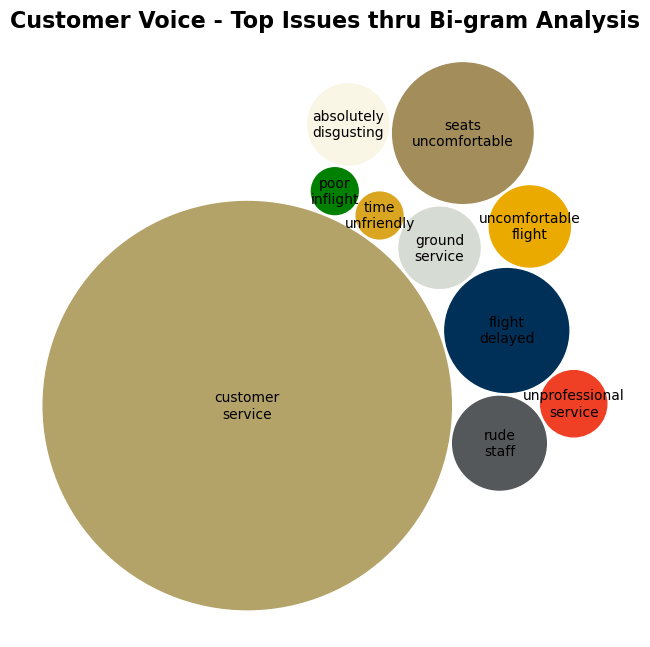
\includegraphics[width=0.5\textwidth]{images/images/bi_gram_analysis.png}
    \caption{Bubble chart representing the Bi-gram Analysis}
    \label{fig:Bigram Analysis}
\end{figure}
Finally, we dive deep into the routes containing the Customer service and Uncomfortable seats issues from Dublin \& Stansted and observe that for Customer Services Issues are more prevalent from Dublin to Edinburg, Amsterdam and Standsted Route. Uncomfortable seats are observed from Stansted to Copenhagen and Dublin route.
\begin{figure}[H]
    \centering
    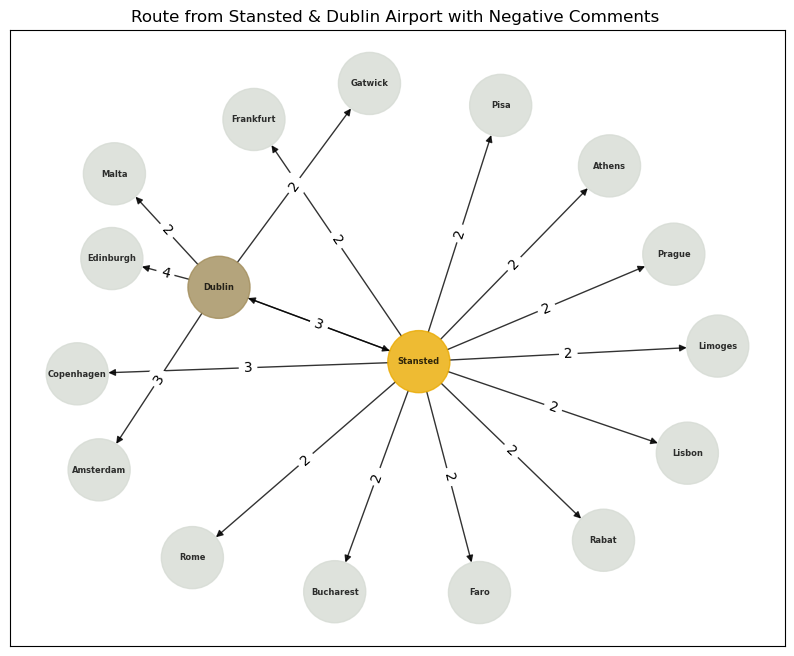
\includegraphics[width=0.7\textwidth]{images/images/route_with_negative_feedback.png}
    \caption{Route Analysis using Network Graph Visualization}
    \label{fig:Route Analysis using Network Graph Visualization}
\end{figure}
\subsection{Sentiment Classifier}
While using pre-trained sentiment classifiers like VADER and spaCy's sentiment analysis module, we observed mis-classifications with negative reviews being tagged as neutrals and positive. So, we manually reviewed and labelled the reviews with positive, negative and neutral sentiment and trained Naive Bayes model to improve accuracy and relevance. We also used it as as a learning opportunities to understanding the intricacies of sentiment analysis using machine learning and build NLP pipelines.

For building the sentiment classifier model, we employed customer review data as feature and sentiment (positive and negative) as label and adopted a standard approach of splitting it into 80\% training and 20\% testing datasets to train and evaluate sentiment analysis classifiers. Utilizing three variants of Naive Bayes classifiers—ComplementNB, MultinomialNB, and BernoulliNB—we trained each model on the training data and evaluated their performance on the test data. Notably, our analysis revealed that the ComplementNB classifier exhibited the highest accuracy of 74.61\% and F1\_Score of 80\%.\\
Performance Metrics on 20\% test dataset:
\begin{table}[H]
\centering
\begin{tabular}{@{}llll@{}}
\toprule
\textbf{Naïve   Bayes Models}        & \textbf{Accuracy} & \textbf{Sensitivity} & \textbf{F1\_Score} \\ \midrule
{\color[HTML]{0D0D0D} ComplementNB}  & 75\%              & 80\%                 & 80\%               \\
{\color[HTML]{0D0D0D} MultinomialNB} & 74\%              & 79\%                 & 80\%               \\
{\color[HTML]{0D0D0D} BernoulliNB}   & 69\%              & 73\%                 & 77\%               \\ \bottomrule
\end{tabular}
\end{table}
\subsection{Final Results \& Recommendation for Ryan Air}
This dissertation set out to examine the role of customer feedback in shaping the operational performance of Ryanair. Through the meticulous collection and categorization of 2248 customer reviews into positive, negative, and neutral sentiments, we employed Spacy's polarity score to conduct sentiment analysis. Our study delved deeper into the negative sentiments expressed in airline reviews, leveraging topic modeling techniques to pinpoint areas generating the most dissatisfaction.

Our findings underscore the critical importance for Ryanair to prioritize enhancements in customer service quality and systematically address specific grievances to safeguard its reputation and cultivate enduring customer loyalty.Our recommendation for Ryanair is to tackle subpar customer service at Dublin airport with priority.


\section{Team Collaboration}
All team-members contributed equally and pro-actively towards the completion of the project.
%Table - Collaboration
\begin{table}[H]
\centering
\begin{tabular}{@{}ll@{}}
\toprule
\textbf{Team   Member} & \textbf{Contribution}                                                                                                                              \\ \midrule
Jagannath Banerjee     & \begin{tabular}[c]{@{}l@{}}Project Formulation \& Strategy, Exploratory Data Analysis, \\ Code Review and Final Project Report Review\end{tabular} \\
Ashish Puri            & Sentiment Analysis, Methodology Review, Final Project Report Review                                                                                \\
Piyush Shivrain        & Topic Modelling, Code Review, Final Project Report Review                                                                                          \\ \bottomrule
\end{tabular}
\end{table}                                  
\section{Bibliography and Credits}
% Your bibliography section
\begin{thebibliography}{5}

    \bibitem{1}
    "Ryanair Passenger Experience Reviews." Www.kaggle.com, \url{www.kaggle.com/datasets/cristaliss/ryanair-reviews-ratings?resource=download. Accessed 11 Mar. 2024}
    
    \bibitem{2}
    TNMT. (n.d.). Passenger Frustration with Airlines. Retrieved from \url{https://tnmt.com/passenger-frustration-with-airlines/}
    
    \bibitem{3}
    Dike, S. E., Davis, Z., Abrahams, A., Anjomshoae, A., \& Ractham, P. (2023, March 21). Evaluation of passengers’ expectations and satisfaction in the airline industry: An Empirical Performance Analysis of online reviews. Benchmarking: An International Journal. \url{https://www.emerald.com/insight/content/doi/10.1108/BIJ-09-2021-0563/full/html} 
    
    
    \bibitem{4}
    Ali, A. (2023, July 13). Airline reviews sentiment analysis by NLP and POWERBI. LinkedIn. \url{https://www.linkedin.com/pulse/airline-reviews-sentiment-analysis-nlp-powerbi-ahmed-ali/} 

    \bibitem{5}
    Blei, D. M., Ng, A. Y., \& Jordan, M. I. (2003, January). Latent dirichlet allocation. Latent Dirichlet Allocation. \url{https://www.jmlr.org/papers/volume3/blei03a/blei03a.pdf} 

    \bibitem{6}
    Jurafsky, D., \& Martin, J. H. (2024, February 3). Naive Bayes, text classifica- tion, and sentiment. Speech and Language Processing. \url{https://web.stanford.edu/~jurafsky/slp3/4.pdf}

    \bibitem{7}
    Edwardes, S. (n.d.). Spacytextblob · spacy universe. spacytextblob. \url{https://spacy.io/universe/project/spacy-textblob} 

    \bibitem{8}
    Sievert, C., \& Shirley, K. E. (2014, June). (PDF) LDAvis: A method for visualizing and interpreting topics. LDAvis: A method for visualizing and interpreting topics. \url{https://www.researchgate.net/publication/265784473_LDAvis_A_method_for_visualizing_and_interpreting_topics} 


    \bibitem{9}
    Zhu, S. (2023, March 6). LDAvis: A deep dive into the popular topic modeling tool. Medium. \url{https://siqi-zhu.medium.com/ldavis-a-deep-dive-into-the-popular-topic-modeling-tool-d0c61a03e969} 


\end{thebibliography}
\end{document}